\documentclass{standalone}
\usepackage{pgfplots}
\pgfplotsset{compat=1.17}

\begin{document}
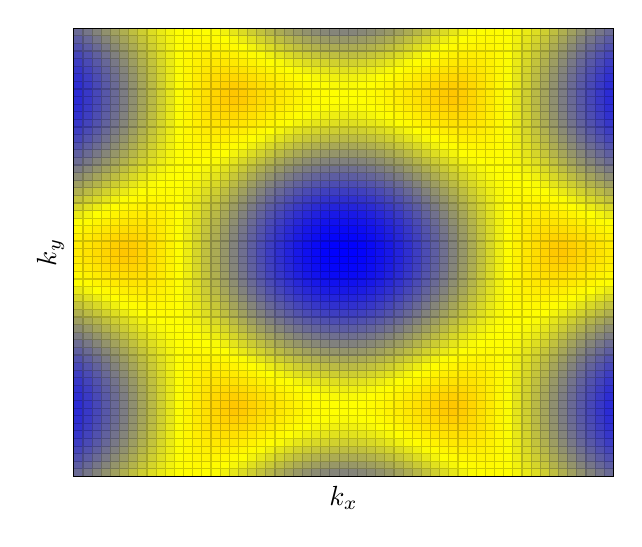
\begin{tikzpicture}
	\begin{axis}[
			% view={20}{10}, % Set the viewing angle
			view={0}{90}, % Set the viewing angle
			xlabel={$k_x$},
			ylabel={$k_y$},
			zlabel={$E$},
			% grid=none, % Turn off the grid
			ticks=none, % Hide ticks
			domain=-3:3,
			ymin=-3, ymax=3,
			% zmin=-5, zmax=3,
		]
		% First surface
		\addplot3[
			surf,
			% colormap/viridis,
			samples=60,
			domain=-3:3,
			y domain=-3:3,
		]
		{sqrt(1 + 4*cos(deg(3*y/2))*cos(deg(sqrt(3)*x/2)) + 4*cos(deg(sqrt(3)*x/2))^2)};

		% Second surface
		\addplot3[
			surf,
			% colormap/thermal,
			samples=60,
			domain=-3:3,
			y domain=-3:3,
		]
		{-sqrt(1 + 4*cos(deg(3*y/2))*cos(deg(sqrt(3)*x/2)) + 4*cos(deg(sqrt(3)*x/2))^2)};
	\end{axis}
\end{tikzpicture}
\end{document}
